%%%%%%%%%%%%%%%%%%%%%%%%%%%%%%%%%%%%%%%%%%%%%%%%%%%%%%%%%%%%%%%%%%%
%                                                                 %
%  GEANT manual in LaTeX form                                     %
%                                                                 %
%  Michel Goossens (for translation into LaTeX)                   %
%  Version 1.00                                                   %
%  Last Mod. Jan 24 1991  1300   MG + IB                          %
%                                                                 %
%%%%%%%%%%%%%%%%%%%%%%%%%%%%%%%%%%%%%%%%%%%%%%%%%%%%%%%%%%%%%%%%%%%
\Documentation{S.Giani, S.Ravndal}
\Submitted{10.03.94}      \Revised{10.03.94}
\Version{Geant 3.21}\Routid{GEOM010}
\Makehead{Tracking inside volumes and optimisation}



The tracking of particles through the geometrical data structure is the key
functionality of {\tt GEANT}. 
At every particle's step, the program must find the
volume where the particle is ({\tt GTMEDI}) and the next boundary it will cross
({\tt GTNEXT}). This can take
about $60\%$ of the total simulation time (even for detectors described
in an optimized way); therefore, a new logic has been introduced to minimize
the time spent for the search in the geometrical tree. 

\section{ Virtual divisions}

Instead of a linear or
binary search (time spent proportional or logarithmic with the number of
volumes, respectively), a `direct access' technique has been developed to
make the time basically independent from the number of volumes. Every volume
containing other volumes is `virtually' divided in equal slices at 
initialization time via the call to {\tt GGCLOS}
(the best axis is computed automatically). 
For each slice,
a data structure is filled with a list of the volumes 
identifiers intersecting such
slice. 
Slices with identical lists are pointing to the same contents
and are collected. At 
tracking time it is immediate to find in which slice the particle is and only
its contents have to be checked. The same is true to find the next boundary to
be crossed: only if the intersection point with a content lies outside the 
current collection of slices, the next one will be checked. The algorithm
gives in average about a factor 2 in speed for the overall simulation in the
large detectors. It also minimizes the dependency of the performance
on the skill and experience of the programmer and allows a fast tracking even
in geometrical structures received from CAD systems.

\section{ Other optimisation tools}

The following facilities are kept for backward compatibility reasons.
If called by the user, these optimisation tools are called at 
initialisation time, but not used at tracking time. Instead, the
new optimisation using 'virtual divisions' is performed.
If the user wants to use the older optimisation tools, he can 
recompile {\tt GEANT} 3.21 using the {\tt PATCHY} flag {\tt +OLD}.
\begin{enumerate}
\item \Rind{GSORD}/\Rind{GGORD}

From the position of the contents inside a given volume, the
subroutine \Rind{GSORD} computes fictitious
boundaries along the specified coordinate, simulating
a division with irregular step size. A binary search technique is used
to identify within which pseudo-cell the current point is. The slow process
of computing whether the point is inside or outside the contents is therefore
limited to the few (if any) volumes overlapping with that
pseudo-cell, as sketched in fig~\ref{fg:geom001-2}.

\begin{figure}[hbt]
      \centering
      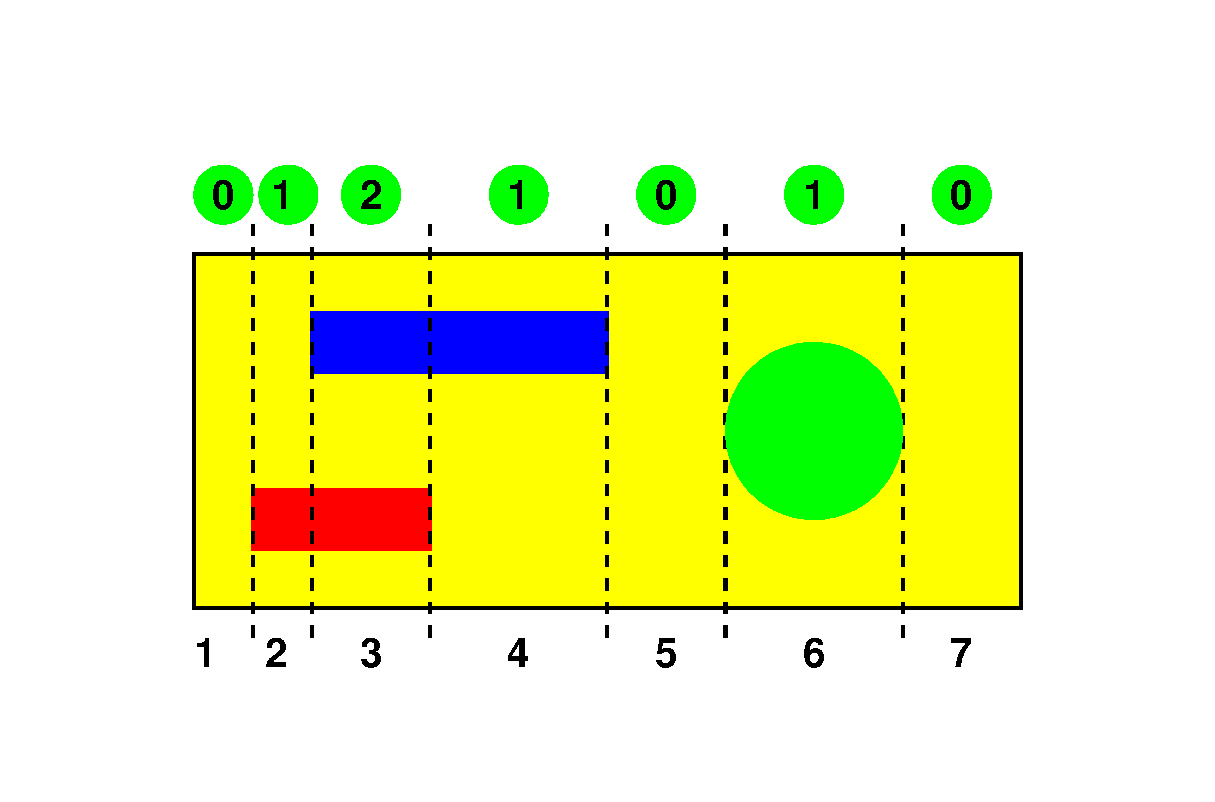
\epsfig{file=eps/geom001-2.eps,width=16cm}
      \caption{Example of pseudo-cells created by {\tt GSORD}}
      \label{fg:geom001-2}
\end{figure}

The coordinate selected for the pseudo division can be any of
{\tt X, Y, Z, $R_{xy}$, $R$, $\phi$ or $\theta$;}.
For a given volume, the call to \Rind{GSORD} has to come after all its first
level contents have been positioned.

\item
\Rind{GSNEXT}/\Rind{GSNEAR}

when a particle exits from a daugther of a 
mother volume, the contents are scanned initially
in the order in which 
they have been positioned, and the user should take care over
the best sequence of \Rind{GSPOS} calls. However, when the particle
{\it  comes back}
inside the mother from any one of the contents, it is
usually possible to limit the search to the neighbour contents.
The subroutines \Rind{GSNEXT}/\Rind{GSNEAR} permit the user to inject, at
initialisation time, for each content
in turn, the list of neighbours to search for.
\Rind{GSNEAR} is recommended, \Rind{GSNEXT} is kept for backward,
compatibility and has a different default option. A proper use of this
facility can reduce the search time significantly.

\item \Rind{GSUNEA}/\Rind{GUNEAR}

The volumes to be checked when exiting from one daughter can depend on 
the direction and position of the exiting particles. To optimise tracking
taking into account these dynamic features, the user can code the
\Rind{GUNEAR} routine, and inform {\tt GEANT} that it has to use it
at tracking time by calling the \Rind{GSUNEA} routine.
\end{enumerate}

